\documentclass[10pt,journal]{book}
\usepackage[utf8x]{inputenc}
\usepackage{subfig}
\usepackage{amsmath,amsthm,amssymb,pifont,makeidx,geometry}
\usepackage{makeidx}
\usepackage{calc}
\usepackage{color}
\usepackage{verbatim}
\usepackage{fancyvrb}
\usepackage[pagebackref=true,breaklinks=true,colorlinks,bookmarks=false]{hyperref}
\usepackage{graphicx}
\usepackage{wasysym,pifont}
\usepackage{ulem}
\definecolor{OliveGreen}{cmyk}{0.64,0,0.95,0.40}
\newcommand{\example}[1]{\framebox[0.95\linewidth][l]{\parbox[t]{.93\linewidth}{\ttfamily \tiny #1}}}
\newcommand{\checkItem}{\textbf{\Pisymbol{wasy}{8}}\hspace{3mm}}
%\newcommand{\command}[1]{\framebox[\textwidth][l]{\parbox[t]{\textwidth}{\tt \$ #1}}}
\newcommand{\command}[1]{\framebox[\textwidth][l]{\tt \$ #1}}
\newcommand{\fileName}[1]{{\tt #1}}
\newcommand{\commandTitle}[1]{\paragraph*{\textbf{#1}}\mbox{ }\\}
\newcommand{\commandName}[1]{\textcolor{red}{\tt #1}}
\newcommand{\optionName}[1]{\textcolor{OliveGreen}{\tt #1}}
\newcommand{\outputName}[1]{\textcolor{blue}{\tt #1}}
\newcommand{\Param}[1]{{\tt #1}}
\newcommand*\OptionsLabel[1]{\optionName{#1}}
\newenvironment{Options}{
    \begin{list}{}{
        \let\makelabel\OptionsLabel\setlength\labelwidth{30pt}%
        \setlength\leftmargin{\labelwidth+\labelsep}}}
    {\end{list}}

\newcounter{thenote}
\newenvironment{note}{\stepcounter{thenote} \noindent \textcolor{red}{\textbf{Note \arabic{thenote}}~:}}{\par}
\newcommand{\warning}[1]{\textcolor{red}{\textbf{Warning~: #1}}}

\bibliographystyle{plain}

\graphicspath{{images/}}
%\DeclareGraphicsRule{.jpg}{eps}{.ps.bb}{`convert #1 ps:-}
%\DeclareGraphicsRule{.gif}{eps}{.ps.bb}{`convert #1 ps:-}
%\DeclareGraphicsRule{.png}{eps}{.ps.bb}{`convert #1 ps:-}

\geometry{width=17cm,height=21.7cm}
\makeindex 

\title{\textbf{\textcolor{blue}{OpenMEEG: Hands-on tutorial}}}
\author{Maureen Clerc\\Alexandre Gramfort \\
        Emmanuel Olivi \\Théo Papadopoulo}
\date{OpenMEEG Version 3.0 \\2013}
\begin{document}

    \maketitle
    \tableofcontents



\chapter{Data format}

OpenMEEG handles several file formats corresponding to different types of objects: vectors, matrices, head geometries, meshes, dipoles, conductivities.

    \section{Vectors and matrices}\mbox{ }\\
    By default, matrices and vectors are stored on disk using a MATLAB file format. Symmetric matrices which are not directly representable in the MATLAB
    format are represented as a MATLAB struct. Other vector/matrices file formats are also supported. Forcing a specific file format is achieved by
    specifying the proper file extension. Matlab extension is {\tt .mat}. Other useful file formats are ASCII (extension {\tt .txt}) which generates
    human readable files, and BrainVisa texture file format (extension {\tt .tex}).
 OpenMEEG's own binary file format (extension {\tt .bin}) is available
    solely for backward compatibility and should be considered as deprecated (as it is subsumed by the MATLAB file format).

    \section{Geometrical model,  mesh and conductivity files}\mbox{ }\\
    {\bf OpenMEEG geometrical models} are described through several files. The toplevel file (generally ending with the extension {\tt .geom}) assembles various
    interface descriptions to build \emph{Domains} corresponding to head tissues. Empty lines or lines beginning with {\tt \#} are non-significant.
    The file must start with a special comment line which allows its identification (see example in Figure~\ref{fig:geom}). 
    Geometrical models globally contain 2 sections, one for describing the interfaces and one for describing the domains.
    In OpenMEEG, we make the following distinction between Mesh and Interface, which is helpful for defining non nested geometries. \\
    "Mesh": a collection of vertices and triangles all connected.\\
    "Interface": a closed mesh.\\
    \begin{figure}[ht!]
    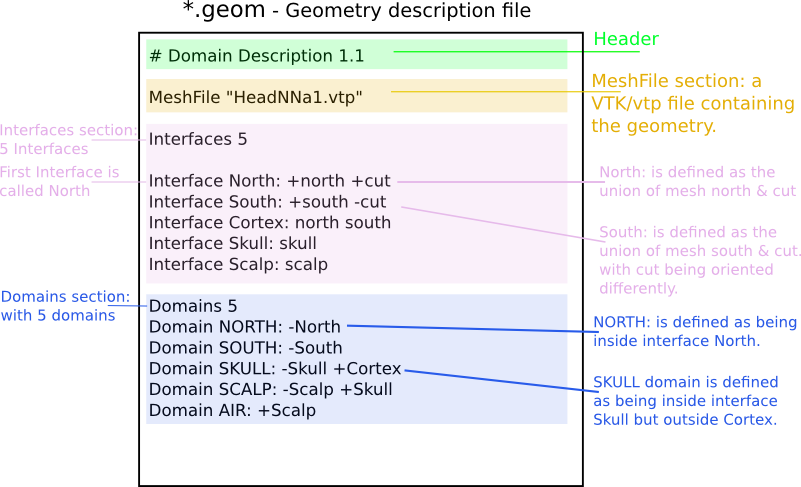
\includegraphics[width=9cm]{geom1.png}
    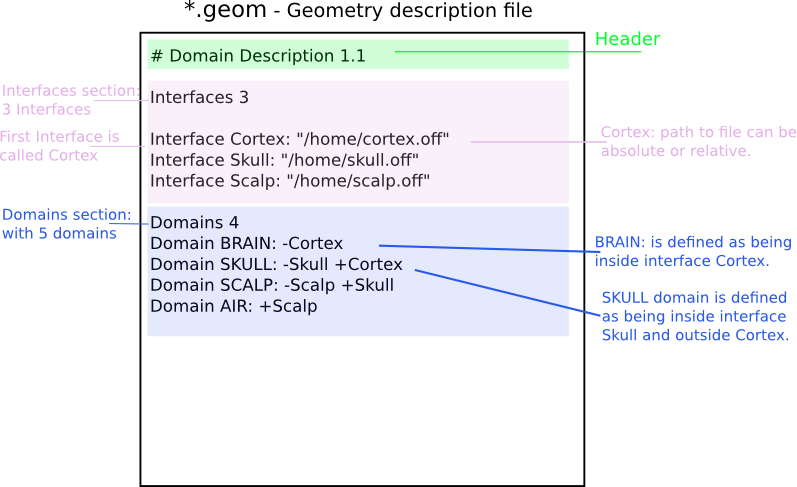
\includegraphics[width=9cm]{geom2.png}
\centerline{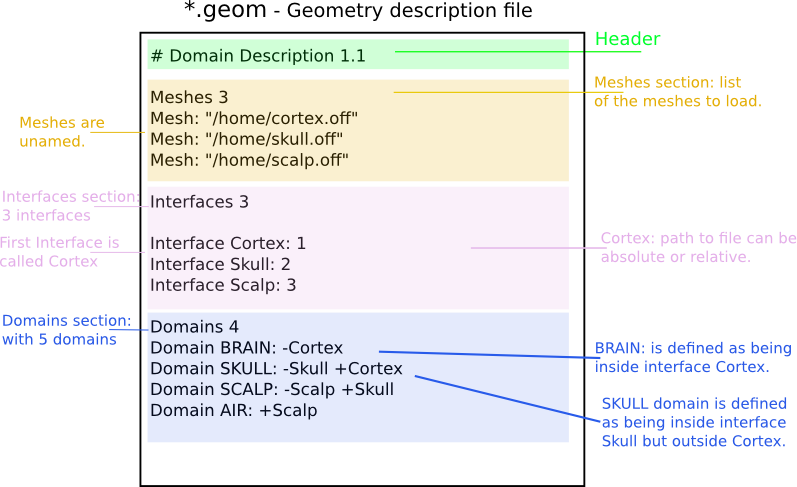
\includegraphics[width=9cm]{geom3.png}}
    \caption{Sample (left) non-nested and (right and bottom) nested geometry descriptions.}
    \label{fig:geom}
    \end{figure}
    \medskip
    The section starting with the keyword {\tt MeshFile} is optional, as well as the section {\tt Meshes}.\\
    If {\tt MeshFile} is found, it specifies the path to the VTK/vtp file containing the vertices and annoted triangles of your geometry. (Triangle annotations are labels that specify the mesh names).\\
    If {\tt Meshes} is found, it specifies the paths to the meshes that may or may not be named. Mesh file formats supported are tri, bnd, mesh, off, and vtk (in case you use VTK).
    A Mesh is defined with the keyword {\tt Mesh} followed by an optional name and "{\tt :}".
    If no name is provided, the Mesh is named by its index (starting from 1).
    
    If none of the two sections {\tt MeshFile} and {\tt Meshes} are present, the next section called {\tt Interfaces} is expected to contain the filenames of the meshes.

    \medskip

    {\tt Interfaces} section specifies the mesh descriptions of the interfaces between tissues. 
    It is introduced by the keyword {\tt Interfaces} followed by the number of such interfaces.

    An Interface is defined with the keyword {\tt Interface} followed by a name and "{\tt :}".
    If no name is provided, the Interface is named by its index (starting from 1).
    If the sections {\tt MeshFile} and {\tt Meshes} were NOT specified before, a path to a mesh file is expected.
    In the opposite case, a sequence of mesh names is expected.

    These meshes are concatenated to form a closed Interface. \\
    '+' or '-' sign preceeding a mesh name reorients the meshes in order to form a consistently oriented interface.

    \medskip

    The second section describes the head tissues and is introduced by the keyword {\tt Domains} followed by the number of such domains.
    Each domain is then described, one domain per line, by the keyword {\tt Domain} followed by the domain name (which serves for identification and also appears in the conductivity description) followed by a list of IDs (names or integers).
    These IDs are the interface names (as depicted in previous paragraph). 
    They must be preceeded by a '+' or '-' sign to indicate whether the domain is outside or inside the corresponding interface (as defined by the outward normal of the interface).
    See Figure~\ref{fig:geom} for a detailed example.

%    For example, in:
%
%    \example{
%        \# Domain Description 1.0\\
%        \\
%        Interfaces 3 Mesh\\
%        \\
%        skull.1.tri\\
%        cortex.1.tri\\
%        scalp.1.tri\\
%        \\
%        Domains 4
%        \\
%        Domain Scalp 1 -3\\
%        Domain Brain -2\\
%        Domain Air 3\\
%        Domain Skull 2 -1
%    }

%    \medskip

%    \noindent
%    the scalp domain (name {\tt Scalp}) is depicted as being outside of the outer skull interface (number 1, file {\tt skull.1.tri}) and inside the outer scalp
%    interface (number 3, file {\tt scalp.1.tri}).

    \bigskip

    {\bf Mesh files} (generally ending with the {\tt .tri} extension) follow the BrainVisa file format for meshes. These files contain two sections. Each section is
    introduced by the character {\tt -} appearing at the beginning of the line followed by a space followed by either one number (first section) or three times
    the same number (second section).

    \medskip

    {\bf The first section} contains a list of points with associated normals. The number on the line introducing the section is the number of points.
    Each following line corresponds to a single point. Its coordinates are the three first numbers appearing on the line. The normal corresponds
    to the following three numbers. Each point is assigned an index (starting at 0) corresponding to its order of appearance in the list.

    \medskip

    {\bf The second section} contains the triangles of the mesh. The number (repeated three times) in the section delimiter corresponds to the number of triangles.
    Each triangle is depicted by a sequence of three integers corresponding to the indices of the points assigned as described in the previous paragraph.

    \medskip

    The following small example describes a very simple mesh containing 4 points and 4 triangles.

    \medskip

    \example{
        - 4\\
        0 0 0 -0.5773 -0.5773 -0.5773\\
        1 0 0 1 0 0\\
        0 1 0 0 1 0\\
        0 0 1 0 0 1\\
        - 4 4 4\\
        0 1 2\\
        0 1 3\\
        0 2 3\\
        1 2 3
    }

    \medskip

    Interfaces are required to be closed in order for the Boundary Element Method to function correctly. This is also necessary for the source meshes when computing forward solutions using surfacic source models (see below). Moreover, the interface meshes must not intersect each other. Non-intersection can be checked with the command \commandName{om\_check\_geom}. The command \commandName{om\_mesh\_info} applied to a mesh provides its number of points, of triangles, minimum and maximum triangle area, and also its Euler characteristic. The Euler characteristic of a closed mesh of genus 0 (homotopic to a sphere) is equal to 2. The Euler characteristic gives an indication if a mesh is likely to be closed or not.\\
    In order to generate a VTK/vtp file, one can use the tool provided \commandName{om\_meshes\_to\_vtp}, which from a list of (closed or not) meshes and names, remove dupplicated vertices and create an easily viewable file in VTK/Paraview.\\
    In order to check a geometry file, one can use the tool provided \commandName{om\_check\_geom}, which display the read informations.

\medskip
    A {\bf conductivity file} (generally ending with the extension {\tt .cond}) is a simple ASCII file that contains associations between tissue names and
    conductivity values. Associations are provided one per line. Empty lines or lines beginning with {\tt \#} are non-significant. The file must start
    with a special comment line which allows its identification. Figure~\ref{fig:cond} provides an example conductivity file corresponding to the geometry file of figure~\ref{fig:geom}.
    \begin{figure}
        \center
        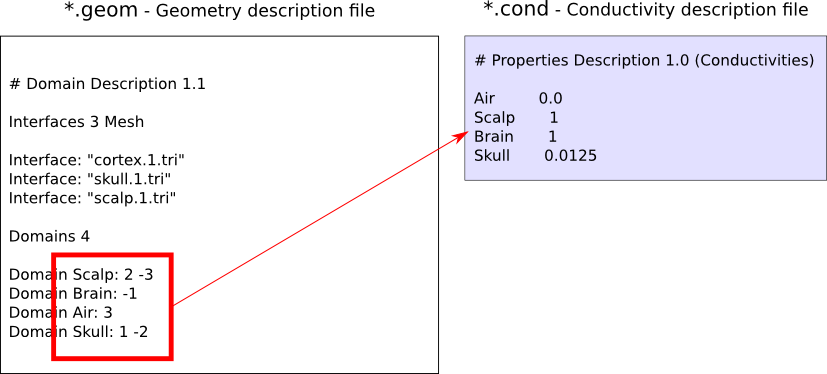
\includegraphics[width=8cm]{cond.png}
        \caption{Sample conductivity file and its correspondance with the geometry file.}
    \label{fig:cond}
    \end{figure}
%Here is a simple example with four tissues.
%    \example{
%        \# Properties Description 1.0 (Conductivities)\\
%        \\
%        Air         0.0\\
%        Scalp       1\\
%        Brain       1\\
%        Skull       0.0125
%    }

    \medskip

    \noindent
    Note that the tissue names are the ones appearing in the Domains descriptions of the file depicting the geometrical model.

    \section{Source descriptions}\mbox{ }\\
    Sources may be represented either by a surfacic distribution of dipoles, or by isolated dipoles.\\
    A {\bf surfacic distribution} can be defined by a mesh that supports the dipoles. The dipole orientations are then constrained to the normal direction to the mesh and the moment amplitude is modelled as continuous across the mesh (piecewise linear). Source values are defined at the mesh vertices.\\
    {\bf Isolated dipoles} are defined by a simple ASCII file as shown in Figure~\ref{fig:dip}.\\

% \AG{}{Source activations are defined in a matrix, whose columns represents a time instant, and each line represents a dipole, indexed with respect to vertex numbering (distributed model) or by dipole number (isolated dipoles).
% }
    \begin{figure}
        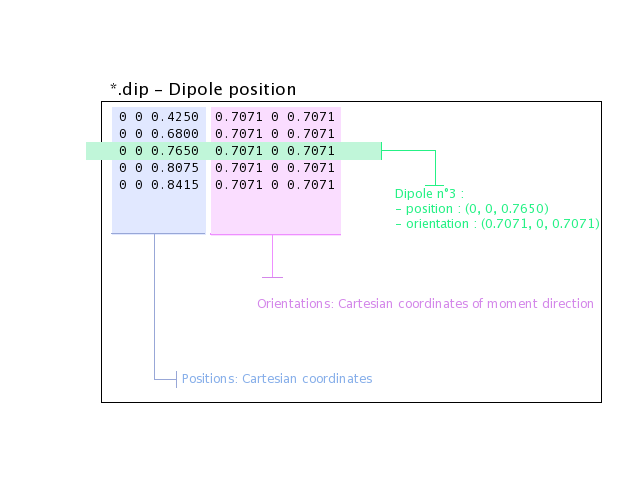
\includegraphics[width=8cm]{dipolePositions_en.png}
        \caption{Sample source description for isolated dipoles.}
        \label{fig:dip}
    \end{figure}
    % \begin{figure}
    %     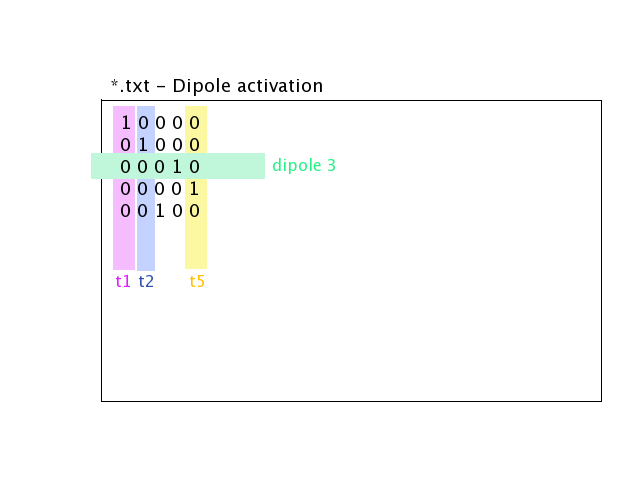
\includegraphics[width=8cm]{dipActiv.png}
    %     \caption{Sample source activation for isolated or distributed dipoles.}
    %     \label{fig:dipactiv}
    % \end{figure}

\chapter{OpenMEEG from the command line} % (fold)
\label{sub:command_line_tools}

\begin{figure}[htbp]
    \centering
        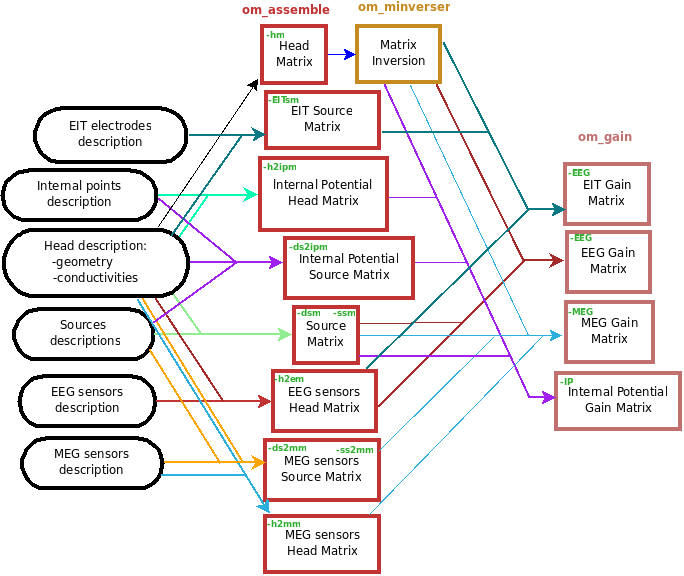
\includegraphics[width=0.95\linewidth]{OpenMEEGSimple}
    \caption{Diagram for the low level pipeline for computing MEG and EEG leadfields (a.k.a., gain matrices) using OpenMEEG.}
    \label{fig:img_OpenMEEGSimple}
\end{figure}


This section reviews the main OpenMEEG command line tools. The general syntax and main options of each command is briefly provided.
Full details are available in OpenMEEG documentation. \emph{In this section, command names are in \commandName{red}, options are in \optionName{green} and produced files are shown in \outputName{blue}.}

    \newpage

    \commandTitle{om\_assemble}
        General syntax:\\[2mm]
        \command{\commandName{om\_assemble} \optionName{Option} \optionName{Parameters} \outputName{Matrix}}\\[2mm]
        This program assembles the different matrices to be used in
        later stages. It uses the head description, the sources and the sensors information. \optionName{Option} selects the type of matrice to assemble.
        \optionName{Parameters} depends on the specific option \optionName{Option}.
        Except if otherwise noted, it takes the form:\\
        \centerline{\Param{subject.geom} \Param{subject.cond} \optionName{OptParam}}\\
        where subject.geom and subject.cond are files describing respectively the geometrical model and the conductivities of the head (see section ???
        for a short description of these files). \optionName{OptParam} depends on the actual \optionName{Option}. \outputName{Matrix} is the name of the output file
        containing the computed matrix.

        We now detail the possible \optionName{Options} (with their abbreviated versions given in parentheses), allowing to define various matrices to assemble:

        \paragraph*{General options for \commandName{om\_assemble}}
            \begin{Options}
                \item[-help] (\optionName{-h},\optionName{--help}):  summarizes all possible options.
            \end{Options}

        \paragraph*{Head modelling options for \commandName{om\_assemble}} produce matrices linked to the propagation of electrical signals in the head.
            \begin{Options}
                \item[-HeadMat] (\optionName{-HM}, \optionName{-hm}): \commandName{om\_assemble} computes the Head matrix for Symmetric BEM (left-hand side
                        of the linear system). This matrix corresponds to the propagation of electrical signals within the head.
                        There is no \optionName{OptParam} in this case.
                         % \optionName{OptParam} is a file describing the internal points.
            \end{Options}

        \paragraph*{Source modelling options for \commandName{om\_assemble}} compute the source matrix for Symmetric BEM (right-hand side of the linear system).
            This matrix maps the representation of the sources to their associated electric potential in an infinite medium ($v_{\Omega_1}$.
            Different options exist for the 2 types of source models:
            \begin{Options}
                \item[-SurfSourceMat] (\optionName{-SSM}, \optionName{-ssm}): should be used for continuous surfacic distributions of dipoles.
                        \optionName{OptParam} is a file containing a mesh that describes the surface.  For faster computations, one can consider giving the name of the domain (containing all dipoles) as a string as an optional parameter in the end of the command line.
                \item[-DipSourceMat] (\optionName{-DSM}, \optionName{-dsm}): should be used when considering several isolated dipoles. This model is the most commonly
                        used and should be used by default even if the dipoles correspond to the vertices of a cortical mesh.
                        \optionName{OptParam} is a file containing the dipole descriptions.  For faster computations, one can consider giving the name of the domain (containing all dipoles) as a string as an optional parameter in the end of the command line (see Exemple).
        % \item[-DipSource2InternalPotMat] (\optionName{-DS2IPM}, \optionName{-ds2ipm}): computes the linear transformation which maps the current dipoles
        %     to the value of the infinite potential at a set of points within a volume.  \optionName{OptParam} should contain two files: a dipole description file, and a file
        %  describing the internal points.

            \end{Options}

        \paragraph*{Sensor modelling options for \commandName{om\_assemble}} compute matrices that integrate source information and computed potentials to
            provide the actual solution of the forward problem. The situation is slightly different for EEG, which only needs to compute the electric potential,
            and for MEG, which depends both on the electric potential and on the sources:
            \begin{Options}
                \item[-Head2EEGMat] (\optionName{-H2EM}, \optionName{-h2em}): \commandName{om\_assemble} computes the interpolation matrix that maps potentials
                        computed on the scalp to EEG sensors. \optionName{OptParam} is a file describing the EEG sensor positions.
                \item[-Head2MEGMat] (\optionName{-H2MM}, \optionName{-h2mm}): \commandName{om\_assemble} computes the contribution of Ohmic currents to the MEG
                        sensors. \optionName{OptParam} is a file describing the SQUIDS geometries and characteristics.
                \item[-Head2InternalPotMat] (\optionName{-H2IPM}, \optionName{-h2ipm}): \commandName{om\_assemble} computes the matrix that allows
                        the computation of potentials at internal positions from potentials and normal currents on head interfaces, as computed by the symmetric BEM.
                \item[-SurfSource2MEGMat] (\optionName{-SS2MM}, \optionName{-ss2mm}): \commandName{om\_assemble} computes the source contribution to the MEG
                        sensors using the same source model as the one used for the option \optionName{-SurfSourceMat}, i.e. surfacic distribution of dipoles.
                        For this option, \optionName{OptParam} takes the form:\\
                        \centerline{\Param{mesh squids}}\\
                        where \Param{mesh} contains a mesh describing the source surface and \Param{squids} is a file describing the SQUIDS geometries
                        and characteristics.
                \item[-DipSource2MEGMat] (\optionName{-DS2MM}, \optionName{-ds2mm}): \commandName{om\_assemble} computes the source contribution to the MEG
                        sensors using the same source model as the one used for the option \optionName{-DipSourceMat}, i.e. isolated dipoles.
                        For this option, \optionName{OptParam} takes the form:\\
                        \centerline{\Param{dipoles squids}}\\
                        where \Param{dipoles} contains the dipole description and \Param{squids} is a file describing the SQUIDS geometries and
                        characteristics.
                \item[-DipSource2InternalPotMat] (\optionName{-DS2IPM}, \optionName{-ds2ipm}): \commandName{om\_assemble} computes the source contribution to the
                        chosen internal points. It gives the potential due to isolated dipoles, as if the medium were infinite.
                        For this option, \optionName{OptParam} takes the form:\\
                        \centerline{\Param{dipoles internalPoints}}\\
                        where \Param{dipoles} contains the dipole description and \Param{internalPoints} is a file describing the points locations.
            \end{Options}

        \paragraph*{EIT options for \commandName{om\_assemble}}
            \begin{Options}
                \item[-EITSourceMat] (\optionName{-EITSM}, \optionName{-EITsm},): \commandName{om\_assemble} computes the right-hand side for scalp current injection.
                        This usage of \commandName{om\_assemble} outputs the right-hand side vector for a given set of EIT electrode.
                        For this option, \optionName{OptParam} is a file describing the EIT electrode positions.\\
                        \\[2mm]
                       
            \end{Options}

    \newpage

    \commandTitle{om\_minverser}
        General syntax:\\[2mm]
        \command{\commandName{om\_minverser} HeadMat \outputName{HeadMatInv}}\\[2mm]
        This program is used to invert the symmetric matrix as provided by the command \commandName{om\_assemble} with the option \optionName{-HeadMat}.
        This command has only one option.
        \begin{Options}
            \item[-help] (\optionName{-h},\optionName{--help}): summarizes the usage of \commandName{om\_minverser}.
        \end{Options}


    \newpage

    \commandTitle{om\_gain}
        General syntax:\\[2mm]
        \command{\commandName{om\_gain} \optionName{Option} HeadMatInv \optionName{Parameters} SourceMat Head2EEGMat \outputName{GainMatrix}}\\

        This command computes the gain matrix by multiplying together matrices obtained previously (e.g. \Param{HeadMatInv} is the matrix computed using
        \commandName{om\_minverser}). The resulting gain matrix is stored in the file \outputName{GainMatrix}.
        \optionName{Option} selects the type of matrice to build. \optionName{Parameters} depend on the specific option \optionName{Option}.
       
        \paragraph*{General options}
            \begin{Options}
                \item[-help] (\optionName{-h},\optionName{--help}): summarizes the usage of \commandName{om\_gain} for all its possible options.
            \end{Options}

        \paragraph*{Gain matrix type options} select the type of gain matrix to be computed by  \commandName{om\_gain}.
            \begin{Options}
                \item[-EEG]: allows to compute an EEG gain matrix.\\
                        \optionName{Parameters} are then:\\
                        \command{\Param{HeadMatInv SourceMat Head2EEGMat}}\\
                        \\
                        \Param{SourceMat} is the matrix obtained using \commandName{om\_assemble} with either of the options \optionName{-SurfSourceMat} or
                        \optionName{-DipSourceMat}, depending on the source model. \Param{Head2EEGMat} is the matrix obtained using \commandName{om\_assemble}
                        with the option \optionName{-Head2EEGMat}. \\
                        \\
                        The \optionName{-EEG} option is also used to compute an  EIT gain matrix: in this case, \Param{SourceMat}
                        should contain the output of the \optionName{-EITsource} option of \commandName{om\_assemble}. Multiplying the EIT gain matrix by the vector of applied currents at each EIT electrode yields the simulated  potential on the EEG electrodes. The applied current on the EIT electrodes should sum to zero.
                \item[-MEG]: allows to compute an MEG gain matrix.\\
            \optionName{Parameters} are then:\\
                        \command{\Param{HeadMatInv SourceMat Head2MEGMat Source2MEGMat}}\\
                        \\
                        \Param{SourceMat} is the matrix obtained using \commandName{om\_assemble} with either of the options \optionName{-SurfSourceMat} or
                        \optionName{-DipSourceMat}, depending on the source model. \Param{Head2MEGMat} is the matrix obtained using \commandName{om\_assemble}
                        with the option \optionName{-HeadMEEGMat}. \Param{Source2MEGMat} is the matrix obtained using \commandName{om\_assemble} with either
                        of the options \optionName{-SurfSource2MEGMat} or \optionName{-DipSource2MEGMat}, depending on the source model.
                \item[-InternalPotential]: allows to compute an internal potential gain matrix for sensors within the volume. \\
                        \optionName{Parameters} are then:\\
                            \command{\Param{HeadMatInv SourceMat Head2InternalPotMat Source2InternalPotMat}}\\
                        \\
                        \Param{Head2InternalPotMat} and \Param{Source2InternalPotMat} are respectivelly obtained using \commandName{om\_assemble} with option
                        \optionName{-Head2InternalPotMat} and \optionName{-DipSource2InternalPotMat}.
            \end{Options}


    \chapter{Examples}

    Assuming a head model represented by the geometry file \Param{head.geom} and the conductivity file \Param{head.cond} and EEG sensors detailed in
    a file \Param{head.eegsensors}.
    Computing the EEG gain matrix for sources distributed on the surface represented
     by the file \Param{sources.tri} is done via the following set of commands:\\

    \example{
        \commandName{om\_assemble} \optionName{-HeadMat} head.geom head.cond \outputName{head.hm}\\
        \commandName{om\_assemble} \optionName{-SSM} head.geom head.cond sources.tri \outputName{head.ssm}\\
        \commandName{om\_assemble} \optionName{-h2em} head.geom head.cond head.eegsensors \outputName{head.h2em}\\
        \commandName{om\_minverser} head.hm \outputName{head.hm\_inv}\\
        \commandName{om\_gain} \optionName{-EEG} head.hm\_inv head.ssm head.h2em \outputName{head.gain}
    }
    \\
    \\
    Considering now isolated dipolar sources detailed in the file \Param{sources.dip} with MEG sensors depicted in the file \Param{head.squids}. Using the same head model, the MEG gain matrix is obtained via the following set of commands:\\

    \example{
        \commandName{om\_assemble} \optionName{-HeadMat} head.geom head.cond \outputName{head.hm}\\
        \commandName{om\_assemble} \optionName{-DSM} head.geom head.cond sources.dip \outputName{head.dsm} "BRAIN"\\
        \commandName{om\_assemble} \optionName{-h2mm} head.geom head.cond head.squids \outputName{head.h2mm}\\
        \commandName{om\_assemble} \optionName{-ds2mm} sources.dip head.squids \outputName{head.ds2mm}\\
        \commandName{om\_minverser} head.hm \outputName{head.hm\_inv}\\
        \commandName{om\_gain} \optionName{-MEG} head.hm\_inv head.dsm head.h2mm head.ds2mm \outputName{head.gain}
    }
\end{document}
